\chapter{宽带调制信号的解调}\label{chap:intro}

% 第五章的撰写思路可以按照以下大纲进行构思,旨在深入讨论宽带亚采样信号的调制解调任务:

% 1. **引言**
%    - 介绍调制解调任务在宽带亚采样信号处理中的重要性和挑战。
%    - 阐述单用户与多用户场景在调制解调任务中的差异和研究的必要性。

% 2. **理论基础**
%    - 回顾调制解调的基本理论,包括宽带信号的亚采样理论。
%    - 描述单用户和多用户场景下信号的特点。

% 3. **调制解调策略**
%    - 针对单用户场景,介绍调制解调的方法及其对应的理论与算法。
%    - 对于多用户场景,探讨在更复杂环境中进行调制解调的策略。

% 4. **实验设计**
%    - 描述用于验证调制解调策略有效性的实验设置,包括数据集描述、评估标准和实验流程。

% 5. **结果分析**
%    - 展示实验结果,分析在单用户和多用户场景中的调制解调性能。
%    - 比较不同调制解调方法的优势和局限性。

% 6. **讨论**
%    - 深入讨论结果背后的原因,提出可能的解释。
%    - 探讨如何优化现有策略,提升调制解调性能。

% 7. **结论与未来工作**
%    - 总结本章的主要发现和对未来技术发展的意义。
%    - 提出后续研究的潜在方向,包括新技术和算法的探索。

% 在整个章节的撰写中,应当重视问题描述的准确性、理论基础的扎实性、实验设计的严谨性以及结果分析的深度。对于单用户和多用户场景,应分别描绘其独特的复杂性,并对应地提出解决策略。同时,也需要考虑到在实际通信系统中应用这些研究成果的可行性和潜在影响。

\section{引言}\label{sec:background}
在第五章中,我们将深入探讨宽带亚采样信号的调制解调任务,这是调制识别研究的一个进阶领域。随着通信技术的不断进步,传统的调制解调方法在处理高速、大容量的通信数据时遇到了瓶颈。特别是在多用户系统中,诸如资源分配和信号干扰等问题使得调制解调任务变得更为复杂。这些挑战呼唤新的解决方案,以提高系统的频谱利用率和通信效率。

在前几章的基础上,我们已经见证了深度学习在调制识别任务中的潜力,特别是在亚采样环境中处理单用户信号时。这为我们提供了启发,即深度学习方法有可能同样适用于更高级的调制解调任务,即使在多用户场景中也是如此。本章的目标是探索和验证深度学习技术在宽带亚采样信号的调制解调任务中的有效性,并解决由多用户共享频谱带来的复杂性问题。

我们将首先回顾宽带亚采样信号处理的理论基础,以及在单用户和多用户场景中进行调制解调的传统方法和相关工作。接着,我们将介绍深度学习在这一领域的应用方法,以及如何通过调整和优化现有的深度学习模型来满足宽带亚采样信号的需求。通过详细的实验设计和结果分析,我们期望为读者提供对这一先进任务的全面理解,并展示深度学习技术在未来通信系统中的应用前景。

\section{宽带单用户调制信号解调}\label{sec:background}

\begin{figure}
    \centering
    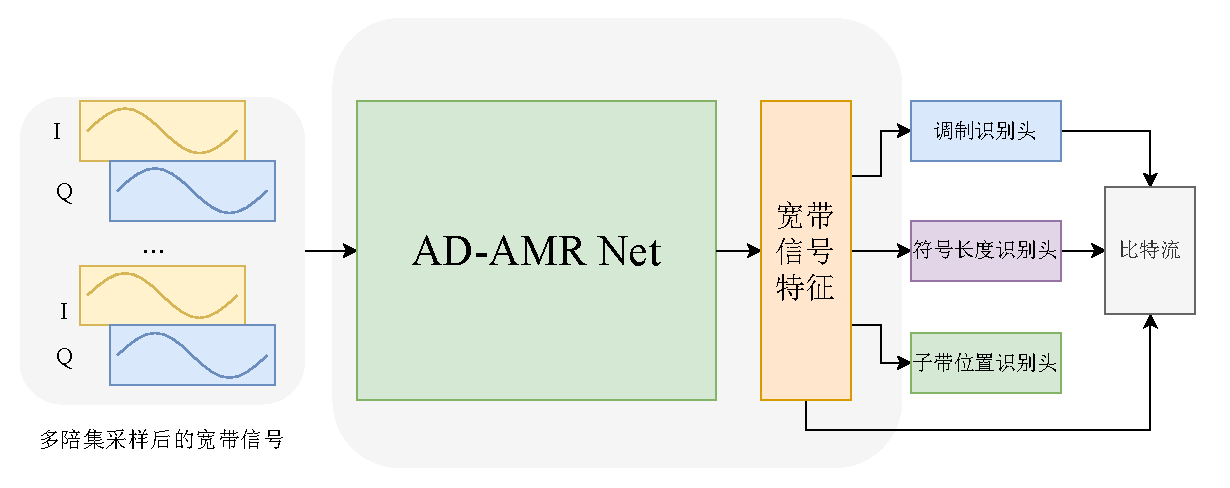
\includegraphics[width=\textwidth]{Image/adamr-wideband_demodulate.pdf}
    \caption{单用户场景下的调制解调流程图}\label{fig:demode_single}
\end{figure}

\section{宽带信号多用户调制信号解调}\label{sec:background}
\begin{figure}
    \centering
    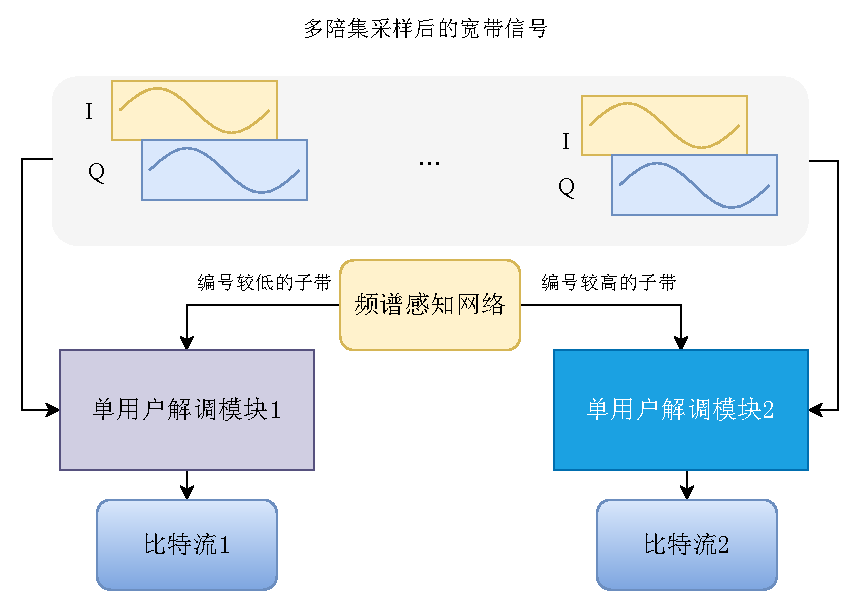
\includegraphics[width=\textwidth]{Image/adamr-wideband_demodulate_mul.pdf}
    \caption{多用户场景下的调制解调流程图}\label{fig:demode_multiple}
\end{figure}

\section{本章总结}\label{sec:background}
\dots
